% @Bab_2.tex
% ==========================================
% BAB II STUDI LITERATUR
% ==========================================
\chapter{STUDI LITERATUR}
\label{chap:studi_literatur}

% --- Machine Learning Operations (MLOps) ---
\section{\textit{Machine Learning Operations} (MLOps)}

\textit{Machine Learning Operations} (MLOps) adalah pendekatan terintegrasi untuk mengelola sistem \textit{machine learning} di lingkungan produksi. Pendekatan ini menggabungkan prinsip DevOps untuk otomasi \textit{deployment} dan operasi perangkat lunak \autocite{devopshandbook2016}, praktik DataOps untuk pengelolaan \textit{pipeline} dan kualitas data, serta \textit{Machine Learning Engineering} untuk pengembangan dan penguatan model. Melalui studi kasus industri, \textcite{paleyes2022challenges} menunjukkan bahwa \textit{deployment} ML menghadirkan tantangan khusus, seperti kerumitan infrastruktur, pengelolaan \textit{dependency} model, dan kebutuhan \textit{monitoring} pada sistem yang bersifat stokastik. Kebutuhan akan MLOps muncul ketika organisasi menuntut kesiapan produksi yang lebih baik, penurunan \textit{technical debt}, serta praktik pengujian dan \textit{monitoring} yang konsisten. \textcite{kreuzberger2023mlops} merumuskan sembilan komponen inti arsitektur MLOps dan kerangka tingkat kematangan yang menegaskan pentingnya integrasi dan otomasi siklus hidup ML bagi keandalan, reproduksibilitas, serta kemudahan pemeliharaan sistem.

Landasan MLOps berangkat dari karakter sistem ML yang berbeda dengan perangkat lunak tradisional karena bergantung pada data dan model yang bersifat stokastik. \textcite{sculley2015hidden} menyoroti bahwa perangkat lunak konvensional bersifat lebih deterministik, sedangkan performa ML sangat dipengaruhi kualitas data pelatihan, \textit{hyperparameter}, dan elemen acak dalam proses pelatihan. Perbedaan ini menambah kompleksitas pada aspek reproduksibilitas, pengujian, \textit{monitoring}, dan \textit{deployment} yang tidak dapat ditangani sepenuhnya oleh praktik DevOps standar. MLOps berperan menjembatani kesenjangan antara eksperimen model dan operasi produksi melalui proses yang terstruktur dan terdokumentasi, sehingga perubahan data maupun kode dapat dikelola secara sistematis dan dampaknya terhadap sistem dapat ditelusuri sepanjang siklus hidup model.

% --- Tingkat Kematangan MLOps ---
\subsection{Tingkat Kematangan MLOps}

Model tingkat kematangan MLOps menggambarkan sejauh mana proses ML di sebuah organisasi telah terotomatisasi dan terintegrasi ke dalam \textit{pipeline} produksi. Berbagai penyedia teknologi menawarkan kerangka kematangan dengan sudut pandang yang berbeda, tetapi semuanya memetakan perjalanan dari proses yang sepenuhnya manual hingga otomasi yang stabil dan dapat diskalakan. Pemetaan ini memberi acuan bagi organisasi untuk menilai posisi saat ini dan merencanakan peningkatan bertahap sesuai kebutuhan sistem dan kesiapan infrastruktur \autocite{googlecloud2024mlops,azure2023maturity,kartakis2022aws,mcknight2020gigaom}. Dengan memahami tingkat kematangan, organisasi dapat menyusun prioritas pengembangan platform dan investasi secara lebih fokus.

Tabel~\ref{tab:mlops_maturity_comparison} menyajikan perbandingan empat kerangka kematangan utama dari Google Cloud, Microsoft Azure, AWS, dan GigaOm. Perbandingan dilakukan pada dimensi DevOps, otomasi \textit{ML pipeline}, integrasi \textit{Continuous Integration}/\textit{Continuous Delivery} (CI/CD), \textit{Continuous Training} (CT), \textit{monitoring} dan \textit{feedback loop}, serta \textit{governance} dan \textit{lineage}. Dimensi tersebut dipilih sebagai indikator praktis untuk menilai struktur dan kedalaman implementasi MLOps di suatu organisasi. Kerangka yang digunakan dalam penelitian ini dipilih secara pragmatis berdasarkan kesesuaian dengan kebutuhan sistem, bukan sebagai standar normatif yang harus diikuti oleh semua organisasi.

{
\footnotesize
\begin{longtable}{|>{\centering\arraybackslash}m{1cm}|>{\centering\arraybackslash}m{0.7cm}|>{\centering\arraybackslash}m{1.3cm}|>{\centering\arraybackslash}m{1.3cm}|>{\centering\arraybackslash}m{1.3cm}|>{\centering\arraybackslash}m{1.5cm}|>{\centering\arraybackslash}m{1.8cm}|>{\centering\arraybackslash}m{1.8cm}|}
\caption{\raggedright Perbandingan Framework Tingkat Kematangan MLOps} \label{tab:mlops_maturity_comparison} \\
\hline
\textbf{FW} & \textbf{L} & \textbf{DevOps Practices} & \textbf{ML Pipeline Automation} & \textbf{CI/CD Integration} & \textbf{CT (Continuous Training)} & \textbf{Monitoring \& Feedback Loop} & \textbf{Governance \& Lineage} \\
\hline
\endfirsthead

\hline
\textbf{FW} & \textbf{L} & \textbf{DevOps Practices} & \textbf{ML Pipeline Automation} & \textbf{CI/CD Integration} & \textbf{CT (Continuous Training)} & \textbf{Monitoring \& Feedback Loop} & \textbf{Governance \& Lineage} \\
\hline
\endhead

\hline
\endfoot

\hline
\endlastfoot

\multirow{3}{=}{\centering\textbf{GCP}} & \textbf{L0} & \cellcolor{red!20}Tidak ada (silo tim) & \cellcolor{red!20}Manual (script, notebook) & \cellcolor{red!20}Tidak ada & \cellcolor{red!20}Tidak ada & \cellcolor{red!20}Tidak ada (\textit{model untracked}) & \cellcolor{red!20}Tidak ada (\textit{no lineage}) \\
\cline{2-8}
& \textbf{L1} & \cellcolor{yellow!20}Parsial (\textit{operational symmetry}) & \cellcolor{green!20}\textbf{Ya} (\textit{end-to-end}) & \cellcolor{yellow!20}Parsial (\textit{pipeline} saja) & \cellcolor{green!20}\textbf{Ya} (\textit{automated}) & \cellcolor{green!20}\textbf{Ya} (\textit{drift detection}) & \cellcolor{green!20}\textbf{Ya} (\textit{metadata store}, \textit{feature store}) \\
\cline{2-8}
& \textbf{L2} & \cellcolor{green!20}\textbf{Ya} (\textit{fully integrated}) & \cellcolor{green!20}\textbf{Ya} (\textit{fully automated}) & \cellcolor{green!20}\textbf{Ya} (CI/CD/CT penuh) & \cellcolor{green!20}\textbf{Ya} (\textit{fully automated}) & \cellcolor{green!20}\textbf{Ya} (\textit{integrated}) & \cellcolor{green!20}\textbf{Ya} (\textit{automated} melalui sistem CI/CD) \\
\hline
\multirow{5}{=}{\centering\textbf{Azure}} & \textbf{L0} & \cellcolor{red!20}Tidak ada (\textit{disparate teams}) & \cellcolor{red!20}Manual (\textit{ad hoc}) & \cellcolor{red!20}Tidak ada & \cellcolor{red!20}Tidak ada & \cellcolor{red!20}Tidak ada (\textit{black box}) & \cellcolor{red!20}Tidak ada (\textit{no tracking}) \\
\cline{2-8}
& \textbf{L1} & \cellcolor{yellow!20}\textbf{Ya} (aplikasi saja) & \cellcolor{red!20}Manual (\textit{model handoff}) & \cellcolor{yellow!20}Aplikasi saja (bukan untuk ML) & \cellcolor{red!20}Tidak ada & \cellcolor{red!20}Minimal (\textit{limited feedback}) & \cellcolor{red!20}Minimal (sulit ditelusuri) \\
\cline{2-8}
& \textbf{L2} & \cellcolor{yellow!20}\textbf{Ya} (DevOps aplikasi) & \cellcolor{green!20}\textbf{Ya} (pelatihan saja) & \cellcolor{red!20}Tidak ada (\textit{release} manual) & \cellcolor{green!20}\textbf{Ya} (pelatihan otomatis) & \cellcolor{yellow!20}Parsial (pelacakan terpusat) & \cellcolor{green!20}\textbf{Ya} (\textit{version control}, manajemen model) \\
\cline{2-8}
& \textbf{L3} & \cellcolor{green!20}\textbf{Ya} (terintegrasi) & \cellcolor{green!20}\textbf{Ya} (latih dan \textit{deploy}) & \cellcolor{green!20}\textbf{Ya} (CD model) & \cellcolor{green!20}\textbf{Ya} (pelatihan otomatis) & \cellcolor{yellow!20}Parsial (\textit{A/B testing}) & \cellcolor{green!20}\textbf{Ya} (pengujian terintegrasi) \\
\cline{2-8}
& \textbf{L4} & \cellcolor{green!20}\textbf{Ya} (\textit{fully integrated}) & \cellcolor{green!20}\textbf{Ya} (\textit{fully automated}) & \cellcolor{green!20}\textbf{Ya} (CI/CD/CT penuh) & \cellcolor{green!20}\textbf{Ya} (\textit{auto retrain}) & \cellcolor{green!20}\textbf{Ya} (\textit{verbose metrics}, \textit{closed loop}) & \cellcolor{green!20}\textbf{Ya} (komprehensif) \\
\hline
\multirow{4}{=}{\centering\textbf{AWS}} & \textbf{Ini-\linebreak tial} & \cellcolor{red!20}Tidak ada & \cellcolor{red!20}Manual (\textit{notebooks}, lokal) & \cellcolor{red!20}Tidak ada & \cellcolor{red!20}Tidak ada & \cellcolor{red!20}Tidak ada & \cellcolor{red!20}Tidak ada (\textit{no standardization}) \\
\cline{2-8}
& \textbf{Rep-\linebreak eat-\linebreak able} & \cellcolor{yellow!20}Parsial (infrastruktur) & \cellcolor{green!20}\textbf{Ya} (\textit{training pipeline}) & \cellcolor{red!20}Tidak ada (\textit{deploy} manual) & \cellcolor{green!20}\textbf{Ya} (\textit{automated}) & \cellcolor{yellow!20}Minimal (infrastruktur eksperimen) & \cellcolor{green!20}\textbf{Ya} (\textit{model registry}, \textit{version control}) \\
\cline{2-8}
& \textbf{Rel-\linebreak iab-\linebreak le} & \cellcolor{green!20}\textbf{Ya} (terintegrasi) & \cellcolor{green!20}\textbf{Ya} (\textit{automated}) & \cellcolor{green!20}\textbf{Ya} (CI/CD terintegrasi) & \cellcolor{green!20}\textbf{Ya} (\textit{automated}) & \cellcolor{green!20}\textbf{Ya} (\textit{prod monitoring}, \textit{rollback}) & \cellcolor{green!20}\textbf{Ya} (IaC, pengujian otomatis) \\
\cline{2-8}
& \textbf{Sca-\linebreak lab-\linebreak le} & \cellcolor{green!20}\textbf{Ya} (multi-\textit{account}/region) & \cellcolor{green!20}\textbf{Ya} (\textit{fully automated}, multi-region) & \cellcolor{green!20}\textbf{Ya} (otomasi penuh) & \cellcolor{green!20}\textbf{Ya} (\textit{auto retrain} melalui \textit{drift detection}) & \cellcolor{green!20}\textbf{Ya} (\textit{drift detection}, optimasi otomatis) & \cellcolor{green!20}\textbf{Ya} (\textit{centralized feature store}, \textit{full governance}) \\
\hline
\multirow{5}{=}{\centering\textbf{Giga Om}} & \textbf{L0} & \cellcolor{red!20}Tidak ada (\textit{no standards}) & \cellcolor{red!20}Manual (inkonsisten) & \cellcolor{red!20}Tidak ada & \cellcolor{red!20}Tidak ada & \cellcolor{red!20}Minimal & \cellcolor{red!20}Minimal (keamanan minimal) \\
\cline{2-8}
& \textbf{L1} & \cellcolor{yellow!20}Parsial (\textit{basic practices}) & \cellcolor{yellow!20}Parsial (sebagian otomatis) & \cellcolor{red!20}Tidak ada (sebagian besar manual) & \cellcolor{red!20}Tidak ada & \cellcolor{yellow!20}Minimal (\textit{basic tracking}) & \cellcolor{yellow!20}Parsial (\textit{limited governance}) \\
\cline{2-8}
& \textbf{L2} & \cellcolor{green!20}\textbf{Ya} (diimplementasikan) & \cellcolor{green!20}\textbf{Ya} (\textit{pipeline} CI/CD) & \cellcolor{green!20}\textbf{Ya} (diimplementasikan) & \cellcolor{yellow!20}Parsial (sebagian otomatis) & \cellcolor{yellow!20}Parsial (\textit{basic monitoring}) & \cellcolor{green!20}\textbf{Ya} (\textit{formal governance} dimulai) \\
\cline{2-8}
& \textbf{L3} & \cellcolor{green!20}\textbf{Ya} (\textit{fully integrated}) & \cellcolor{green!20}\textbf{Ya} (\textit{fully automated}) & \cellcolor{green!20}\textbf{Ya} (komprehensif) & \cellcolor{green!20}\textbf{Ya} (\textit{automated}) & \cellcolor{green!20}\textbf{Ya} (\textit{comprehensive monitoring/alerting}) & \cellcolor{green!20}\textbf{Ya} (\textit{automated governance}, \textit{self-service}) \\
\cline{2-8}
& \textbf{L4} & \cellcolor{green!20}\textbf{Ya} (\textit{fully adaptive}) & \cellcolor{green!20}\textbf{Ya} (\textit{AI-optimized}) & \cellcolor{green!20}\textbf{Ya} (\textit{self-optimizing}) & \cellcolor{green!20}\textbf{Ya} (\textit{continuous learning}) & \cellcolor{green!20}\textbf{Ya} (\textit{continuous learning} dari produksi) & \cellcolor{green!20}\textbf{Ya} (platform terintegrasi dan adaptif penuh) \\
\end{longtable}
}

\vspace{-0.5cm}

\textbf{Keterangan:}
\vspace{0.5em}

\begin{enumerate}
    \item \colorbox{red!20}{Merah}: Tidak ada implementasi atau sepenuhnya manual
    \item \colorbox{yellow!20}{Kuning}: Implementasi parsial atau terbatas
    \item \colorbox{green!20}{Hijau}: Implementasi penuh atau otomatis
    \vspace{0.5em}
\end{enumerate}

Dalam penelitian ini, \textbf{framework Google Cloud digunakan sebagai rujukan utama} untuk mengarahkan implementasi MLOps. Kerangka tiga tingkat (0--2) yang ditawarkan menitikberatkan pada otomasi \textit{end-to-end} dan memberikan definisi yang jelas mengenai CI, CD, dan CT. Kerangka tersebut dirancang untuk organisasi yang membangun sistem ML dari awal dan menempatkan CT sebagai komponen penting sejak Level~1. Penekanan ini membuat hubungan antara perubahan data produksi dan siklus pelatihan model menjadi eksplisit sehingga relevan dengan karakter data finansial yang non-stasioner dan mudah berubah. Gambar~\ref{fig:mlops_level_0} sampai dengan Gambar~\ref{fig:mlops_level_2} mengilustrasikan arsitektur referensi Google Cloud MLOps Level~0 hingga Level~2 yang dijadikan acuan pemetaan kebutuhan platform pada penelitian ini.

\vspace{0.5em}
\begin{enumerate}
    \item \textbf{Level 0: \textit{Manual Process}}

    \begin{figure}[H]
    \centering
    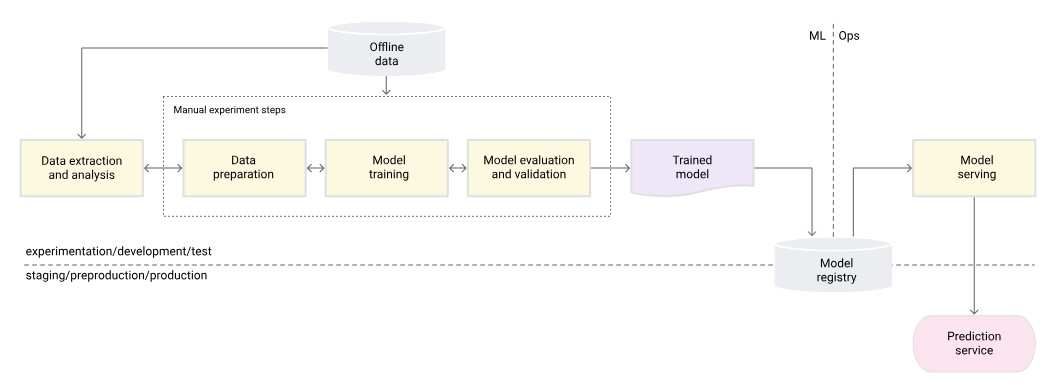
\includegraphics[width=\textwidth]{figures/MLOps_0.jpg}
    \caption{Arsitektur Google Cloud MLOps Level 0}
    \label{fig:mlops_level_0}
    \end{figure}

    Pada Level~0, pengembangan model dan proses \textit{deployment} masih dilakukan secara manual tanpa dukungan \textit{pipeline} otomatis. Tim \textit{data scientist} dan tim operasional bekerja dalam \textit{silo} sehingga koordinasi sangat bergantung pada komunikasi informal dan prosedur tidak baku. CI/CD maupun CT belum tersedia, dan model biasanya dibangun melalui \textit{notebook} atau skrip yang tidak terdokumentasi dengan baik. Kondisi ini menyulitkan pengulangan eksperimen, meningkatkan risiko kesalahan manusia, dan menghambat penskalaan ketika kompleksitas sistem bertambah.

    \vspace{0.5em}

    \item \textbf{Level 1: \textit{ML Pipeline Automation}}

    \begin{figure}[H]
    \centering
    
\includegraphics[width=\textwidth]{figures/MLOps_1.jpg}
    \caption{Arsitektur Google Cloud MLOps Level 1}
    \label{fig:mlops_level_1}
    \end{figure}

    Pada Level~1, organisasi mulai menerapkan otomasi \textit{pipeline} ML secara \textit{end-to-end}. Otomasi ini umumnya mencakup validasi data, \textit{feature engineering}, pelatihan, validasi model, dan pelatihan ulang otomatis berdasarkan jadwal tertentu. \textit{Tracking} eksperimen dan \textit{metadata} mulai dipusatkan sehingga iterasi pemodelan menjadi lebih cepat dan keputusan teknis dapat ditelusuri. Model dideploy sebagai layanan prediksi, dan sistem mulai memantau \textit{data drift} maupun \textit{model drift} secara lebih terstruktur. Integrasi CI/CD dan CT pada tahap ini masih terbatas dan belum sepenuhnya menyatu dengan praktik rekayasa perangkat lunak yang lebih luas.

    \vspace{0.5em}

    \item \textbf{Level 2: \textit{CI/CD Pipeline Automation}}

    \begin{figure}[H]
    \centering
    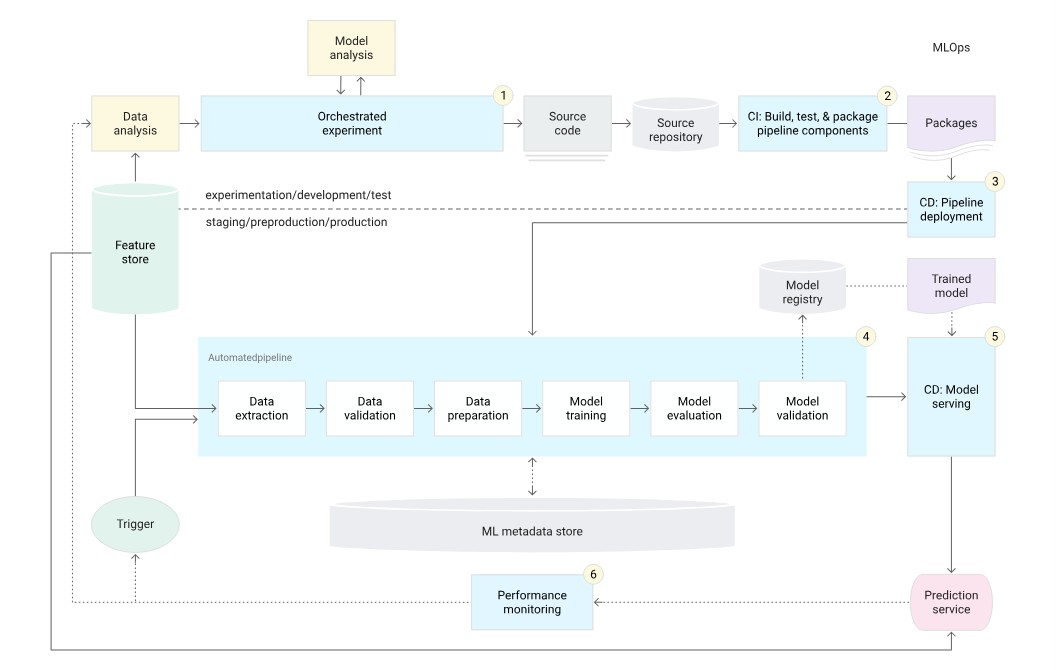
\includegraphics[width=\textwidth]{figures/MLOps_2.jpg}
    \caption{Arsitektur Google Cloud MLOps Level 2}
    \label{fig:mlops_level_2}
    \end{figure}
    
    Pada Level~2, seluruh \textit{pipeline} ML dikelola oleh CI/CD yang terotomatisasi dan terintegrasi untuk pengujian data, model, dan kode. CI, CD, dan CT berjalan sebagai satu rangkaian yang utuh, termasuk \textit{automated retraining} yang dipicu oleh \textit{feedback loop} dari produksi dan metrik bisnis. Level ini juga mencakup praktik \textit{governance} yang kuat melalui proses \textit{approval}, \textit{compliance check}, dan pengaturan hak akses yang jelas. Selain itu, terdapat \textit{proactive monitoring} untuk metrik ML seperti \textit{data drift}, \textit{concept drift}, dan degradasi kinerja model \autocite{googlecloud2024mlops}. Dengan struktur ini, perubahan di lingkungan produksi dapat direspons melalui aksi otomatis yang terukur dan terdokumentasi.
\end{enumerate}

Berdasarkan kerangka kematangan tersebut, penelitian ini menargetkan implementasi MLOps pada \textbf{Level 2: \textit{CI/CD Pipeline Automation}}. Pada tingkat ini, sistem mencakup \textit{automated ML pipeline}, CT yang aktif, integrasi CI/CD penuh, pengelolaan \textit{metadata} terpusat, serta \textit{monitoring} yang terhubung dengan \textit{alerting} dan mekanisme pemicu otomatis. Tingkat kematangan ini sejalan dengan kebutuhan sistem perdagangan finansial yang menuntut kualitas data dan model tetap konsisten sepanjang siklus hidup sistem, sekaligus mempermudah penerapan \textit{continuous improvement} berbasis data.

% --- Komponen Inti Arsitektur DataOps dan MLOps ---
\subsection{Komponen Inti Arsitektur DataOps dan MLOps}

Arsitektur DataOps dan MLOps tersusun dari sekumpulan komponen yang bersama-sama menopang siklus hidup sistem ML dari hulu ke hilir. Pemahaman yang jelas terhadap fungsi dan interaksi setiap komponen menjadi dasar untuk merancang sistem yang dapat diskalakan dan mudah dipelihara. Integrasi yang tepat membantu mengurangi risiko kegagalan di produksi dan mempercepat transisi dari eksperimen ke \textit{deployment}, sehingga kemampuan analitik dapat diselaraskan dengan kebutuhan bisnis tanpa mengorbankan stabilitas operasional.

\textbf{Komponen \textit{Data Management}} bertanggung jawab mengelola data mulai dari \textit{ingestion}, validasi, \textit{versioning}, hingga penyimpanan. \textcite{polyzotis2018data} menunjukkan bahwa masalah pada siklus hidup data sering menjadi sumber kegagalan sistem ML di produksi. \textit{Data validation} memastikan data mengikuti \textit{schema} yang disepakati dan memenuhi standar kualitas, sedangkan \textit{data versioning} menyimpan \textit{snapshot dataset} agar eksperimen dapat direproduksi dan dianalisis ketika terjadi anomali. Pada arsitektur yang diusulkan, komponen ini diperkuat oleh kombinasi \textit{streaming platform}, \textit{object storage}, dan alat validasi kualitas data yang terintegrasi dalam satu alur.

\textbf{Komponen \textit{Feature Engineering}} mengubah data mentah menjadi fitur yang siap digunakan model. Tantangan utama tahap ini adalah menjaga keselarasan logika dan data antara pelatihan dan \textit{serving} untuk menghindari \textit{training--serving skew}. \textit{Feature Store} menyediakan repositori terpusat yang menyimpan definisi dan nilai fitur sehingga dapat diakses kembali oleh \textit{training pipeline} maupun \textit{serving}. Bagian~\ref{sec:feature_store} membahas \textit{Feature Store} secara lebih rinci karena komponen ini berperan langsung dalam menjaga validitas temporal dan konsistensi fitur. Dengan repositori terpusat, tim dapat mengurangi duplikasi logika dan mempermudah audit perubahan fitur.

\textbf{Komponen \textit{Model Training}} mencakup pemilihan algoritme, pengaturan \textit{hyperparameter}, dan pelaksanaan proses pelatihan. Praktik MLOps menekankan \textit{experiment tracking} yang mencatat parameter, \textit{dataset}, versi kode, konfigurasi infrastruktur, dan metrik hasil pelatihan. Pada skala besar, \textit{distributed training} memerlukan orkestrasi khusus yang dibahas pada Bagian~\ref{sec:kubeflow}. Keluaran proses pelatihan dihubungkan dengan \textit{model registry} untuk pengelolaan versi sehingga setiap model yang dihasilkan memiliki konteks dan rekam jejak yang jelas.

\textbf{Komponen \textit{Model Analysis} dan validasi} memastikan model memenuhi standar kualitas sebelum dipromosikan ke produksi. Tahap ini meliputi evaluasi metrik, perbandingan dengan \textit{baseline} atau \textit{champion model}, serta analisis tambahan seperti \textit{fairness}, \textit{robustness}, dan \textit{interpretability}. Hasil evaluasi menjadi dasar keputusan apakah model layak digunakan atau perlu disesuaikan. Integrasi tahap analisis ke dalam \textit{pipeline} membantu menurunkan risiko penerapan model yang tidak stabil di lingkungan nyata dan memudahkan pembuktian kualitas model kepada pemangku kepentingan.

\textbf{Komponen \textit{Deployment} dan \textit{Model Serving}} menangani penyajian model sebagai layanan prediksi. Infrastruktur \textit{serving} harus mampu memberikan latensi rendah, \textit{throughput} tinggi, skala elastis, dan \textit{high availability}. Strategi seperti \textit{canary release} dan \textit{A/B testing} membantu peluncuran model baru secara bertahap dan aman. \textcite{fowler2014microservices} menunjukkan bahwa pola \textit{microservices} sesuai untuk pemisahan tanggung jawab dan \textit{rollout} bertahap. Implementasi KServe sebagai komponen utama \textit{model serving} di atas Kubernetes dijelaskan pada Bagian~\ref{sec:kserve} dan diintegrasikan dengan komponen lain dalam platform MLOps.

\textbf{Komponen \textit{Monitoring} dan \textit{Observability}} memantau kesehatan sistem dan kinerja model saat berjalan di produksi. Pemantauan mencakup metrik sistem seperti latensi, \textit{throughput}, dan \textit{error rate}, serta metrik ML seperti distribusi fitur, distribusi prediksi, dan \textit{confidence score}. Deteksi \textit{data drift} dan \textit{concept drift} menjadi penting \autocite{bayram2022concept} karena degradasi kinerja sering terjadi secara bertahap dan tidak langsung terlihat dari metrik infrastruktur. \textit{Monitoring} perlu terhubung dengan \textit{feedback loop} otomatis agar pelatihan ulang dapat dipicu ketika degradasi teridentifikasi. Pada arsitektur penelitian ini, metrik dari \textit{Feature Store}, \textit{stream processing}, dan \textit{model serving} dikumpulkan oleh \textit{monitoring stack} yang akan dijelaskan pada Bagian~\ref{sec:prometheus_grafana}.

\textbf{Komponen \textit{Governance} dan \textit{Compliance}} memastikan praktik ML sejalan dengan kebijakan organisasi, regulasi, dan prinsip etika \autocite{bernardo2024data}. \textcite{stoyanovich2020responsible} menyoroti pentingnya \textit{lineage tracking}, \textit{access control}, dan \textit{audit logging} untuk menjaga akuntabilitas. Pada sektor finansial, \textit{governance} yang kuat menjadi prasyarat sebelum sistem ML dioperasikan secara luas. Dalam implementasi, konsep tersebut diwujudkan melalui platform \textit{metadata management} seperti DataHub yang digabungkan dengan lapisan autentikasi dan otorisasi terpusat serta manajemen rahasia yang aman. Aspek ini dibahas lebih lanjut pada Bagian~\ref{sec:governance} sebagai bagian dari fondasi DataOps dan MLOps yang tepercaya.

% --- Kubernetes untuk ML Workloads ---
\section{Kubernetes untuk \textit{Machine Learning Workloads}}
\label{sec:kubernetes}

Kubernetes telah berkembang menjadi \textit{de facto standard} untuk \textit{container orchestration} \autocite{lakka2025kubernetes} dan banyak dimanfaatkan untuk menjalankan \textit{workload} ML. \textcite{kreuzberger2023mlops} menunjukkan bahwa Kubernetes mendominasi implementasi MLOps modern baik di industri maupun penelitian. Kubernetes menyediakan fondasi deklaratif untuk \textit{deploying}, \textit{scaling}, dan \textit{managing} aplikasi, termasuk \textit{workload} ML yang memerlukan komputasi intensif dan dinamis. Dengan pendekatan deklaratif, keadaan klaster yang diinginkan didefinisikan melalui \textit{manifest} dan dipertahankan oleh \textit{control plane}, sehingga replikasi lingkungan menjadi lebih mudah dan konfigurasi manual yang rentan kesalahan dapat dikurangi.

\textbf{Portabilitas} Kubernetes memungkinkan \textit{workload} dalam bentuk kontainer dijalankan secara konsisten di lingkungan \textit{on-premise}, \textit{public cloud}, maupun \textit{edge}. \textcite{adusumilli2025serverless} menegaskan bahwa abstraksi ini menurunkan hambatan transisi dari pengembangan ke produksi dan mendukung strategi \textit{hybrid} atau \textit{multi-cloud}. \textbf{Skalabilitas} Kubernetes penting untuk \textit{training} dan \textit{serving} yang kebutuhan sumber dayanya dapat berubah dengan cepat. \textit{Horizontal Pod Autoscaler} menyesuaikan jumlah \textit{pod} berdasarkan metrik, sedangkan \textit{Cluster Autoscaler} mengatur jumlah \textit{node} agar kapasitas klaster selaras dengan beban dan biaya tetap terkendali. Kombinasi fitur tersebut menjadikan Kubernetes fondasi yang fleksibel untuk platform MLOps yang terukur.

\textbf{\textit{Resource management}} dan isolasi di Kubernetes memungkinkan skenario \textit{multi-tenant} dikelola secara aman dan adil. \textit{Namespaces}, \textit{resource quota}, dan \textit{limit range} mengatur pemakaian sumber daya oleh setiap tim atau aplikasi, sedangkan \textit{device plugin} mengelola penjadwalan \textit{Graphics Processing Unit} (GPU) untuk \textit{workload} pelatihan dan inferensi berat. Fitur \textit{priority} dan \textit{preemption} memastikan \textit{workload} kritis tetap berjalan meskipun sumber daya sedang terbatas. Pendekatan GitOps memanfaatkan Kubernetes sebagai \textit{control plane} yang dikonfigurasi melalui deklarasi di repositori Git. Alat seperti Argo~CD memantau repositori Git (termasuk yang di-host di Gitea) dan menyelaraskan keadaan klaster dengan \textit{manifest} yang didefinisikan. Pola ini memperkuat praktik CI/CD dan audit konfigurasi, dan akan dibahas pada Bagian~\ref{sec:gitops}.

% --- Arsitektur Kubernetes ---
\subsection{Arsitektur Kubernetes}

Sebuah klaster Kubernetes terdiri dari \textit{control plane} dan satu atau lebih \textit{worker node}. \textit{Control plane} mencakup \textit{API server}, \textit{etcd}, \textit{scheduler}, dan \textit{controller manager} yang bersama-sama menjaga \textit{desired state} klaster. \textit{API server} berfungsi sebagai gerbang utama untuk seluruh interaksi dengan klaster, baik dari pengguna maupun komponen internal. \textit{Etcd} menyimpan \textit{state} klaster secara konsisten sehingga setiap perubahan konfigurasi dapat disinkronkan dengan andal. \textit{Scheduler} memilih \textit{node} yang akan menjalankan \textit{pod}, sedangkan \textit{controller manager} menjalankan loop rekonsiliasi untuk memastikan kondisi aktual mengikuti spesifikasi.

Di sisi lain, \textit{worker node} menjalankan \textit{kubelet}, \textit{container runtime}, dan \textit{kube-proxy}. Untuk \textit{workload} ML, \textit{node} sering dilengkapi GPU dan memori besar, sehingga pelabelan \textit{node} dan pengaturan kendala \textit{scheduling} menjadi penting. Konsep \textit{node pool} memungkinkan pengelompokan \textit{node} berdasarkan spesifikasi sumber daya, sehingga organisasi dapat menyeimbangkan kebutuhan kinerja dengan efisiensi biaya. Pemahaman terhadap komponen arsitektur ini membantu perancang sistem ML memanfaatkan Kubernetes secara optimal, khususnya saat mengatur prioritas \textit{job} pelatihan dan layanan inferensi yang peka terhadap latensi dan harus tetap tersedia.

% --- Kubernetes Primitives ---
\subsection{Kubernetes \textit{Primitives} untuk \textit{Machine Learning}}

\textit{Pod} merupakan unit terkecil \textit{deployment} yang dapat memuat \textit{model server} dan \textit{sidecar} seperti \textit{logger} dan \textit{metrics exporter}. \textit{Deployment} sesuai untuk layanan \textit{inference} yang bersifat \textit{stateless}, sedangkan \textit{StatefulSet} digunakan untuk \textit{workload} yang memerlukan identitas dan penyimpanan persisten. Dengan memanfaatkan kedua pola ini, layanan inferensi dan komponen data dapat diatur secara terpisah namun tetap terkoordinasi dalam satu klaster yang sama. Pola tersebut memudahkan pengelolaan siklus hidup layanan tanpa mengganggu komponen lain.

\textit{Job} dan \textit{CronJob} mendukung \textit{batch workload} seperti pelatihan berkala atau prediksi massal yang terjadwal. \textit{ConfigMap} dan \textit{Secret} memisahkan konfigurasi dan data sensitif dari \textit{image}, sehingga pengelolaan konfigurasi \textit{pipeline} lebih aman dan tidak mengharuskan pembangunan ulang \textit{image} saat konfigurasi berubah. \textit{Service} dan \textit{Ingress} menyediakan \textit{endpoint} stabil di dalam dan di luar klaster, dan mengatur rute HTTP/HTTPS untuk aplikasi. Dalam konteks \textit{inference}, konfigurasi yang tepat pada komponen ini penting agar akses ke model tetap andal dan terlindungi, termasuk integrasi dengan \textit{Application Programming Interface} (API) \textit{gateway} dan mekanisme autentikasi di lapisan luar.

% --- Feature Store dan Feast ---
\section{\textit{Feature Store} dan Feast}
\label{sec:feature_store}

\textit{Feature Store} adalah komponen penting MLOps yang menyediakan mekanisme terpusat untuk mengelola dan \textit{serving} fitur secara konsisten. Tanpa repositori terpusat, fitur cenderung dihitung dan diakses dengan cara berbeda antara pelatihan dan \textit{serving}, sehingga memicu \textit{training--serving skew}. \textit{Feature Store} mengatasi masalah ini dengan menyediakan definisi, penyimpanan, dan penyajian fitur menggunakan logika yang sama di seluruh siklus hidup ML. Selain itu, \textit{Feature Store} memperkaya \textit{metadata} fitur yang dapat dimanfaatkan untuk \textit{governance} dan audit, sehingga proses penelusuran dan penjelasan fitur menjadi lebih mudah.

Feast merupakan salah satu \textit{open-source Feature Store} yang banyak diadopsi \autocite{feast2024}. Proyek ini awalnya dikembangkan oleh Gojek dan menawarkan arsitektur \textit{dual-store} untuk memisahkan fitur historis di \textit{offline store} dan fitur terkini di \textit{online store}. Desain Feast menekankan fleksibilitas dan kemudahan integrasi dengan infrastruktur data yang telah ada di organisasi. Dengan pendekatan ini, Feast dapat diterapkan pada berbagai kombinasi \textit{stack} data modern tanpa memaksa perubahan arsitektur yang drastis. Posisi Feast dalam arsitektur penelitian ini menjadi penghubung antara \textit{pipeline} data, penyimpanan, dan layanan \textit{serving}.

% --- Komponen Arsitektur Feast ---
\subsection{Komponen Arsitektur Feast}

\textbf{\textit{Feature Registry}} menyimpan definisi fitur, \textit{feature view}, dan sumber data sebagai \textit{metadata} terpusat. \textit{Registry} biasanya diletakkan di repositori Git sehingga mendukung \textit{version control} dan praktik GitOps \autocite{limoncelli2022gitops}. Selain definisi teknis, \textit{registry} juga memuat tipe data, batasan, \textit{owner}, dan dokumentasi yang relevan. Informasi ini meningkatkan \textit{discoverability} dan \textit{governance} fitur serta memudahkan audit perubahan definisi, sehingga evolusi fitur dapat dikelola secara lebih terkontrol.

\textbf{\textit{Offline Store}} digunakan untuk melayani fitur historis yang dibutuhkan pada pelatihan atau \textit{batch inference}. Pada penelitian ini, ClickHouse dipilih sebagai \textit{offline store} (Bagian~\ref{sec:clickhouse}). Feast melakukan \textit{point-in-time correct join} antara \textit{feature view} dan \textit{entity timestamp} untuk mencegah kebocoran temporal. \textbf{\textit{Online Store}} menyediakan fitur berlatensi rendah untuk \textit{real-time inference}. Redis Stack digunakan sebagai \textit{online store} (Bagian~\ref{sec:redis}). Fitur dapat dimaterialisasikan secara terjadwal dari \textit{offline store} atau dialirkan \textit{real-time} dari \textit{streaming pipeline}. Pemisahan \textit{offline} dan \textit{online} ini memungkinkan setiap lapisan dioptimalkan sesuai pola beban tanpa mengorbankan konsistensi definisi fitur.

% --- Feature Materialization ---
\subsection{\textit{Feature Materialization} dan \textit{Point-in-Time Correctness}}

\textit{Feature materialization} adalah proses menghitung nilai fitur dan menuliskannya ke \textit{Feature Store}. Feast mendukung \textit{batch materialization} terjadwal untuk data historis dan \textit{stream materialization} secara \textit{real-time} dari sumber seperti Kafka (Bagian~\ref{sec:kafka}). Kombinasi kedua pendekatan ini memungkinkan organisasi menyesuaikan strategi pemrosesan dengan kebutuhan \textit{freshness} fitur. Dengan demikian, fitur yang sama dapat dimanfaatkan secara konsisten untuk pelatihan maupun inferensi tanpa logika yang terpecah di berbagai layanan.

\textbf{\textit{Point-in-time correctness}} memastikan bahwa fitur historis hanya dibangun dari data yang benar-benar tersedia pada waktu tertentu. Properti ini sangat penting pada data \textit{time-series} karena kesalahan waktu dapat menimbulkan kebocoran informasi masa depan ke masa lalu. \textcite{polyzotis2018data} menekankan bahwa kebocoran temporal merupakan salah satu penyebab utama penurunan kinerja model ketika masuk ke produksi. Feast menerapkan prinsip ini melalui \textit{join} berbasis \textit{entity key} dan \textit{event timestamp} sehingga integritas temporal tetap terjaga. Dengan mekanisme ini, evaluasi dan \textit{backtesting} di domain finansial dapat memberikan gambaran performa yang lebih realistis terhadap kondisi dunia nyata.

% --- Feature Serving dan Retrieval ---
\subsection{\textit{Feature Serving} dan \textit{Retrieval}}

Feast menyediakan \textit{feature retrieval} melalui Python SDK atau gRPC API untuk pola \textit{online} maupun \textit{batch}. \textit{Online retrieval} mengambil nilai fitur terbaru dari \textit{online store} dengan latensi rendah dan cocok untuk \textit{real-time inference}. \textit{Batch retrieval} mengambil fitur historis dari \textit{offline store} untuk pelatihan atau prediksi dalam volume besar. Konsistensi antara kedua pola ini mengurangi duplikasi logika perhitungan fitur dan menekan \textit{technical debt} yang timbul akibat implementasi ad hoc, sehingga tim data dapat mengandalkan satu sumber kebenaran untuk definisi dan perhitungan fitur.

\textit{Feature transformation} memungkinkan penerapan transformasi saat pengambilan fitur dilakukan. Melalui \textit{on-demand transformation}, \textit{derived feature} dihitung ketika \textit{retrieval} berlangsung sehingga nilai fitur tetap \textit{fresh} tanpa memperbesar beban penyimpanan. Mekanisme ini mendukung iterasi desain fitur yang lebih cepat dan fleksibel karena perubahan logika transformasi dapat diterapkan tanpa perlu mengulang proses materialisasi besar. Pendekatan ini juga mempermudah penyelarasan antara eksplorasi data di tahap riset dan kebutuhan operasional di produksi.

% --- Manajemen Siklus Hidup Model ---
\section{Manajemen Siklus Hidup Model}
\label{sec:model_lifecycle}

Manajemen siklus hidup model mencakup tahapan pengembangan, \textit{deployment}, \textit{monitoring}, pemeliharaan, hingga \textit{decommissioning}. Pengelolaan yang terstruktur memastikan model di produksi tetap akurat, stabil, dan relevan dengan perubahan data maupun kebutuhan bisnis. Selain itu, pengaturan siklus hidup yang jelas membantu organisasi menjelaskan keputusan yang diambil oleh sistem otomatis kepada pemangku kepentingan dan regulator. Pada domain finansial, kemampuan menjelaskan proses pengambilan keputusan ini menjadi penting untuk menjawab pertanyaan terkait risiko dan kepatuhan.

Di samping menjaga kualitas teknis, manajemen siklus hidup model juga berfungsi memastikan kesesuaian dengan kebijakan internal dan regulasi eksternal. Platform DataOps dan MLOps menyediakan alat untuk mengotomatisasi alur promosi model, pencatatan \textit{metadata}, dan kontrol perubahan. Dengan adanya otomasi tersebut, setiap tahap dalam siklus hidup model dapat ditelusuri dan diaudit kembali jika diperlukan. Pendekatan ini mengurangi risiko \textit{model drift}, kesalahan konfigurasi, dan penggunaan model yang sudah tidak sesuai dengan kondisi terkini di lapangan.

% --- MLflow ---
\subsection{MLflow untuk \textit{Experiment Tracking} dan \textit{Model Registry}}
\label{sec:mlflow}

MLflow merupakan standar \textit{open-source} yang banyak digunakan untuk pengelolaan siklus hidup ML \autocite{mlflow2024}. \textbf{MLflow Tracking} mencatat parameter, metrik, \textit{tag}, dan \textit{artifact} untuk setiap eksperimen sehingga variasi pendekatan pemodelan dapat dibandingkan secara sistematis. Kemampuan ini memudahkan tim untuk mengidentifikasi konfigurasi yang memberikan hasil terbaik tanpa kehilangan jejak eksperimen sebelumnya. Dukungan \textit{autologging} untuk berbagai \textit{framework} umum dan \textit{manual logging} untuk kebutuhan khusus menjadikan pencatatan eksperimen lebih fleksibel dan dapat disesuaikan dengan pola kerja tim data.

Antarmuka \textit{user interface} (UI) MLflow mempermudah penelusuran \textit{run}, perbandingan metrik, dan pengunduhan \textit{artifact} sehingga eksperimen dapat dikelola secara terstruktur dan mudah direproduksi. \textbf{MLflow Model Registry} mengelola versi model, status siklus hidup, dan menjadi titik serah antara pelatihan dan \textit{deployment}. Mekanisme \textit{versioning} memungkinkan beberapa versi model hidup berdampingan sehingga \textit{rollout} dan \textit{A/B testing} dapat dilakukan secara terkendali. Promosi model antartahap dapat diotomatisasi melalui integrasi CI/CD dan praktik GitOps, dengan anotasi dan \textit{tag} yang memperkaya konteks pada setiap versi model yang disimpan.

\textbf{MLflow Models} menyediakan format pengemasan model yang portabel lintas berbagai infrastruktur \textit{serving}. Dalam skenario produksi, MLflow umumnya diintegrasikan dengan alat \textit{serving} khusus seperti KServe (Bagian~\ref{sec:kserve}) sehingga model dapat dijalankan pada lingkungan yang terstandar. Untuk menyimpan \textit{artifact}, MLflow membutuhkan \textit{object storage}; dalam arsitektur penelitian ini, MinIO dipakai sebagai \textit{artifact store} (Bagian~\ref{sec:minio}). Dengan konfigurasi ini, seluruh artefak pelatihan dapat disimpan secara terpusat, tahan lama, dan mudah ditelusuri kembali ketika diperlukan evaluasi atau audit.

% --- Kubeflow ---
\subsection{Kubeflow untuk Orkestrasi \textit{ML Pipeline}}
\label{sec:kubeflow}

Kubeflow dirancang untuk menyederhanakan orkestrasi \textit{workflow} ML di atas Kubernetes agar tetap portabel dan mudah diskalakan \autocite{kubeflow2024}. \textbf{Kubeflow Pipelines} memungkinkan definisi dan eksekusi \textit{pipeline} multi-langkah yang diterjemahkan menjadi Argo \textit{Workflow} dan dijalankan di dalam klaster. Setiap \textit{pipeline} terdiri dari \textit{component} yang dikontainerisasi dengan \textit{input--output} eksplisit sehingga alur data dan \textit{dependency} antar langkah dikelola secara otomatis. Pendekatan ini mengurangi kompleksitas skrip orkestrasi manual dan membuat proses lebih mudah direproduksi.

\textbf{Kubeflow Pipelines UI} menyediakan tampilan untuk melacak \textit{run}, membandingkan hasil, melihat \textit{lineage}, serta menjadwalkan \textit{recurring run} untuk tugas seperti pelatihan ulang atau \textit{batch inference}. \textbf{Kubeflow Notebooks} menawarkan lingkungan Jupyter di Kubernetes sehingga eksperimen dapat memanfaatkan sumber daya klaster, termasuk GPU, tanpa konfigurasi manual yang rumit. \textbf{Kubeflow Training Operator} menyediakan \textit{Custom Resource Definition} (CRD) seperti \textit{TFJob} dan \textit{PyTorchJob} untuk menjalankan \textit{distributed training job} secara terkelola. Dengan kombinasi komponen ini, Kubeflow memposisikan Kubernetes sebagai platform utama untuk menjalankan \textit{ML pipeline} dalam skala produksi.

% --- Alternative Orchestration Tools ---
\subsection{Alternatif Platform Orkestrasi}
\label{sec:orchestration_alternatives}

Selain Kubeflow, terdapat sejumlah platform lain yang relevan untuk orkestrasi ML dan data. \textbf{Apache Airflow} adalah orkestrator matang berbasis \textit{Directed Acyclic Graph} (DAG) yang mendukung penjadwalan kompleks, banyak integrasi, dan berbagai \textit{executor} termasuk \textit{KubernetesExecutor}. Keunggulan Airflow terletak pada fleksibilitas dan kemampuan \textit{error handling} untuk \textit{data pipeline} yang melibatkan banyak sistem berbeda. Banyak organisasi memanfaatkannya sebagai tulang punggung orkestrasi data pada \textit{data warehouse} dan \textit{data lake}.

Beberapa platform seperti \textbf{Optimus} memanfaatkan Airflow sebagai basis dan menambahkan lapisan abstraksi untuk memudahkan orkestrasi transformasi data secara deklaratif dan standar. Pendekatan ini membantu mengelola dependensi, kualitas data, dan jadwal eksekusi untuk \textit{warehouse} dan \textit{data lake} secara konsisten. \textbf{Tekton Pipelines} menawarkan CI/CD \textit{cloud-native} berbasis CRD yang \textit{vendor-agnostic}. Dalam konteks MLOps, Tekton dapat digunakan untuk mengotomatisasi alur mulai dari \textit{code commit} hingga \textit{deployment} model di klaster. Pemilihan orkestrator bergantung pada kebutuhan dan konteks organisasi, dan kombinasi beberapa platform tetap memungkinkan selama integrasi dan batas tanggung jawabnya diatur secara jelas.

% --- KServe ---
\subsection{KServe untuk Penyajian Model}
\label{sec:kserve}

KServe merupakan platform \textit{Kubernetes-native} untuk \textit{serverless inference} yang menyediakan \textit{auto-scaling} dan strategi \textit{deployment} lanjutan \autocite{kserve2024}. KServe berstatus \textit{incubating} di CNCF dan dibangun di atas Knative, sehingga memanfaatkan kemampuan \textit{scale-to-zero} dan pengelolaan lalu lintas bawaan dari ekosistem tersebut. \textbf{\textit{InferenceService}} menjadi CR utama yang menggambarkan model, \textit{runtime}, kebutuhan sumber daya, dan strategi \textit{deployment} yang digunakan. Melalui satu definisi deklaratif, tim dapat mengatur cara model dijalankan, diskalakan, dan diekspos.

\textbf{\textit{Predictor}} menjalankan proses \textit{inference} dengan dukungan bawaan untuk berbagai \textit{framework}, serta \textit{custom predictor} jika diperlukan. \textbf{\textit{Transformer}} memungkinkan \textit{preprocessing} dan \textit{postprocessing} sebagai layanan terpisah, sedangkan \textbf{\textit{Explainer}} menyediakan fungsi interpretabilitas seperti Anchor, LIME, atau SHAP. KServe juga mendukung \textit{canary deployment} dan \textit{A/B testing} untuk meluncurkan model baru secara bertahap sambil memantau dampaknya. Pembagian trafik dan kemampuan \textit{rollback} yang cepat menjadikan penerapan model di produksi lebih aman, terutama ketika diintegrasikan dengan \textit{observability stack} untuk memantau kualitas layanan secara berkelanjutan.

% --- Data Processing dan Streaming ---
\section{Pemrosesan dan \textit{Streaming} Data}
\label{sec:data_processing}

Infrastruktur pemrosesan data bertugas mengubah data mentah menjadi fitur yang siap digunakan untuk pelatihan maupun \textit{inference}. Sistem perlu mendukung \textit{batch processing} untuk data historis dan \textit{stream processing} untuk komputasi fitur secara \textit{real-time}. Integrasi antara pemrosesan, orkestrasi, dan \textit{Feature Store} membentuk alur hulu--hilir yang konsisten, sehingga definisi fitur dan \textit{training dataset} dapat dikelola sebagai sasaran bersama dan perubahan di hulu dapat ditelusuri dampaknya sampai ke model produksi.

Pada studi kasus perdagangan saham dan kripto, pemrosesan \textit{batch} dibutuhkan untuk membangun \textit{training dataset} historis yang representatif, sementara \textit{streaming} digunakan untuk menghasilkan fitur yang peka terhadap waktu. Selain \textit{engine} pemrosesan seperti Apache Spark dan Apache Flink, arsitektur penelitian ini memanfaatkan ekosistem alat \textit{open-source} seperti Kafka dan komponen pendukungnya (misalnya Raccoon \autocite{raystack2025raccoon}, Stencil \autocite{raystack2025stencil}, Firehose \autocite{raystack2025firehose}, serta Optimus dan Dagger \autocite{raystack2025optimus,raystack2025dagger}). Alat-alat ini digunakan untuk menyederhanakan proses \textit{ingest}, transformasi, dan distribusi data sehingga pengelolaan aliran data dapat dilakukan secara standar dan dapat diaudit.

% --- Apache Spark ---
\subsection{Apache Spark untuk \textit{Batch Processing}}
\label{sec:spark}

Apache Spark menyediakan \textit{engine} terpadu untuk \textit{batch processing}, SQL, dan analitik berskala besar. \textcite{zaharia2016spark} menjelaskan bahwa Spark berbasis pada RDD yang terdistribusi, \textit{immutable}, dan toleran kesalahan melalui mekanisme \textit{lineage}. Karakteristik ini memungkinkan pemrosesan data besar secara andal dan mempermudah pengulangan komputasi ketika terjadi kegagalan. Dengan abstraksi yang konsisten, tim data dapat menggunakan antarmuka yang sama untuk berbagai jenis beban kerja analitik.

\textbf{Spark SQL} menggunakan \textit{DataFrame} dan optimasi otomatis sehingga kueri analitik besar dapat dijalankan dengan efisien. \textbf{Spark MLlib} menyediakan algoritme ML terdistribusi yang bermanfaat untuk \textit{baseline}, \textit{feature pipeline}, ataupun pelatihan skala besar tanpa perlu membangun infrastruktur tambahan. Integrasi Spark dengan Kubernetes memungkinkan \textit{executor} dijalankan sebagai \textit{pod} yang elastis dan dapat diskalakan. Spark \textit{Operator} menyediakan CRD sehingga aplikasi Spark dapat dikelola secara deklaratif dan konsisten dengan pendekatan GitOps yang diterapkan pada komponen lain.

Dalam arsitektur penelitian ini, Spark dihubungkan dengan Feast untuk menulis fitur hasil pemrosesan \textit{batch} ke ClickHouse (Bagian~\ref{sec:clickhouse}). Di tingkat orkestrasi, lapisan seperti Optimus \autocite{raystack2025optimus} dapat dimanfaatkan untuk mendefinisikan \textit{job} Spark dan transformasi data secara deklaratif. Lapisan ini juga membantu mengatur dependensi, jadwal eksekusi, dan pengujian kualitas data sehingga praktik DataOps yang sistematis dan terukur dapat diterapkan pada jalur pemrosesan \textit{batch}.

% --- Apache Flink ---
\subsection{Apache Flink untuk \textit{Stream Processing}}
\label{sec:flink}

Apache Flink dirancang untuk komputasi \textit{stateful stream} dengan jaminan \textit{exactly-once} dan latensi rendah. \textcite{carbone2015apache} menjelaskan bahwa Flink memproses data secara kontinu tanpa menunggu akumulasi, namun tetap mendukung \textit{batch} sebagai kasus khusus. Pendekatan ini sangat sesuai untuk data \textit{tick} finansial yang terus mengalir dan memerlukan respons cepat. Dengan model pemrograman yang konsisten, tim data dapat merancang \textit{pipeline} yang sama untuk pemrosesan terus-menerus maupun perhitungan agregat.

\textbf{\textit{State management}} Flink menjaga konsistensi komputasi meskipun terjadi kegagalan, melalui \textit{keyed state} atau \textit{operator state}. \textbf{\textit{Event time processing}} dengan \textit{watermark} memungkinkan analitik yang akurat meskipun data datang terlambat, sementara dukungan \textit{windowing} memfasilitasi perhitungan berbagai metrik teknikal secara \textit{real-time} untuk fitur. Integrasi Flink dengan Kafka menyediakan \textit{end-to-end exactly-once semantics} melalui \textit{checkpointing}. Flink juga dapat menulis fitur langsung ke Redis Stack sebagai \textit{online feature store} melalui Feast (Bagian~\ref{sec:redis}), sedangkan kerangka konfigurasi seperti Dagger \autocite{raystack2025dagger} menyederhanakan definisi \textit{job} Flink yang digunakan berulang pada berbagai skenario.

% --- Apache Kafka ---
\subsection{Apache Kafka untuk \textit{Event Streaming}}
\label{sec:kafka}

Apache Kafka merupakan \textit{event streaming platform} yang lazim digunakan untuk membangun \textit{real-time data pipeline} \autocite{apachekafka2024}. \textcite{kleppmann2017ddia} menekankan bahwa model \textit{event log} Kafka mendukung \textit{throughput} tinggi, latensi rendah, dan \textit{durability}. Desain partisi dan replikasi yang digunakan membuat Kafka cocok sebagai tulang punggung \textit{streaming} pada perdagangan berfrekuensi tinggi dan \textit{event-driven architecture}. Dengan struktur tersebut, data dapat dialirkan secara terukur ke berbagai konsumen tanpa bergantung pada integrasi khusus yang rapuh.

\textbf{\textit{Topic}} membagi \textit{event} ke dalam partisi agar konsumsi dapat dilakukan secara paralel, dengan replikasi untuk toleransi kesalahan. \textit{Producer} dan \textit{Consumer} API mendukung berbagai jaminan pengiriman, dan \textit{consumer group} memungkinkan konsumsi paralel yang terukur. \textbf{Kafka Connect} menyediakan \textit{connector} siap pakai untuk mengalirkan data dari dan ke sistem eksternal sehingga Kafka dapat menghubungkan proses \textit{ingest}, pemrosesan, dan \textit{Feature Store} dalam alur yang konsisten. Pada implementasi praktis, kolektor peristiwa seperti Raccoon \autocite{raystack2025raccoon} dan \textit{schema registry} ringan seperti Stencil \autocite{raystack2025stencil} membantu menjaga evolusi \textit{message schema} tetap tertata. \textit{Sink service} seperti Firehose \autocite{raystack2025firehose} memudahkan penulisan \textit{stream} ke berbagai tujuan tanpa perlu membangun integrasi khusus berulang kali.

% --- Storage Systems ---
\section{Sistem Penyimpanan}
\label{sec:storage}

Lapisan penyimpanan harus mampu melayani kueri historis untuk pelatihan sekaligus \textit{lookup} berlatensi rendah untuk \textit{online serving}. Selain itu, penyimpanan juga perlu menampung \textit{artifact} besar seperti model, \textit{checkpoint}, dan dataset mentah. Karena tidak ada satu sistem yang optimal untuk seluruh pola akses, arsitektur modern cenderung menggunakan beberapa jenis penyimpanan yang berbeda. Dengan memisahkan beban kerja analitik, \textit{serving}, dan \textit{object storage}, setiap jenis beban dapat dioptimalkan secara terpisah tanpa saling mengganggu.

Dalam penelitian ini, ClickHouse digunakan sebagai \textit{offline feature store}, Redis Stack sebagai \textit{online feature store} sekaligus \textit{vector store}, dan MinIO sebagai \textit{object storage} \autocite{clickhouse2024,redis2024,minio2024}. Kombinasi tersebut dipilih agar kebutuhan \textit{throughput}, latensi, dan kapasitas penyimpanan pada konteks perdagangan finansial dapat terpenuhi. Bagian-bagian berikut menguraikan karakteristik masing-masing sistem dan perannya dalam arsitektur yang diusulkan sehingga pemetaan peran dapat disesuaikan dengan pola penggunaan sebenarnya di sistem.

% --- ClickHouse ---
\subsection{ClickHouse sebagai \textit{Offline Feature Store}}
\label{sec:clickhouse}

ClickHouse adalah DBMS kolumnar \textit{open-source} yang dioptimalkan untuk \textit{Online Analytical Processing} (OLAP) pada volume data besar \autocite{clickhouse2024}. Format kolumnar sangat sesuai untuk kueri analitik yang membaca banyak baris namun hanya membutuhkan sejumlah kolom, sehingga I/O dan penggunaan memori dapat ditekan. Fitur kompresi ClickHouse memanfaatkan \textit{codec} kolumnar untuk mengurangi ukuran data dan pada saat yang sama meningkatkan kinerja kueri.

\textit{Query engine} ClickHouse menggunakan eksekusi tervektorisasi dan paralelisme kueri untuk memaksimalkan pemanfaatan CPU. \textit{Partitioning} dan \textit{sparse index} mendukung \textit{data pruning} sehingga kueri tetap efisien ketika dataset bertumbuh besar. Sebagai \textit{offline store} Feast, ClickHouse menyimpan fitur historis untuk penyusunan \textit{training dataset}. \textit{Materialization job} menulis fitur ke tabel ClickHouse, sementara \textit{point-in-time correct join} dijalankan di atas kemampuan kuerinya sehingga kebutuhan validitas temporal dapat dipenuhi tanpa menambah kerumitan besar di lapisan aplikasi.

% --- Redis Stack ---
\subsection{Redis Stack untuk \textit{Online Feature Store} dan Pencarian Vektor}
\label{sec:redis}

Redis Stack memperluas Redis dengan modul seperti RedisJSON, RedisTimeSeries, RedisBloom, dan RedisSearch sehingga mendukung \textit{full-text} dan \textit{vector similarity search} \autocite{redis2024}. Kombinasi modul-modul ini memungkinkan Redis Stack berfungsi sebagai \textit{online feature store} sekaligus \textit{vector database} berlatensi rendah yang relevan untuk \textit{real-time inference} di sistem perdagangan dengan tuntutan \textit{Service Level Agreement} (SLA) ketat. Dalam arsitektur ini, Redis Stack menjadi titik utama \textit{online retrieval} untuk fitur tabular maupun berbasis \textit{embedding}.

\begin{enumerate}
    \item \textbf{Arsitektur \textit{Vector Database} dan Pengindeksan}

    \textit{Vector database} menyimpan dan mengambil \textit{embedding} berdimensi tinggi secara efisien, lengkap dengan \textit{metadata} yang dapat dimanfaatkan untuk \textit{filtering} dan \textit{governance}. Dengan memanfaatkan indeks \textit{Approximate Nearest Neighbor} (ANN), pencarian kemiripan dapat melayani permintaan dalam jumlah besar tanpa melanggar SLA latensi. \textbf{Algoritme Hierarchical Navigable Small Worlds (HNSW)} \autocite{malkov2020efficient} membangun graf berlapis yang menyeimbangkan kecepatan dan akurasi. Parameter seperti $M$, \textit{efConstruction}, dan \textit{ef} mengatur \textit{trade-off} antara akurasi, latensi, dan konsumsi memori sehingga pemilihannya perlu disesuaikan dengan profil \textit{workload}.

    \item \textbf{Jenis dan Karakteristik \textit{Embedding}}

    \textit{Embedding} yang digunakan pada sistem produksi dapat berupa \textit{sparse embeddings} untuk pencarian leksikal, \textit{dense embeddings} untuk pencarian semantik, maupun \textit{quantized embeddings} untuk efisiensi memori. \textit{Product Quantization} \autocite{jegou2011product} menawarkan kompromi antara efisiensi penyimpanan dan mutu hasil pencarian. Pemilihan jenis \textit{embedding} bergantung pada sifat sinyal yang dimanfaatkan, seperti teks berita, percakapan di media sosial, atau sinyal teknikal yang diturunkan dari pergerakan harga.

    \item \textbf{Implementasi Produksi Redis Stack}

    Redis Stack sebagai \textit{online store} Feast menyediakan \textit{feature retrieval} berlatensi rendah untuk \textit{real-time inference}. Fitur dapat dimaterialisasikan dari ClickHouse atau dialirkan langsung dari \textit{pipeline} Flink--Kafka sesuai kebutuhan \textit{freshness}. Redis mendukung mekanisme persistensi \textit{Redis Database} (RDB) dan \textit{Append-Only File} (AOF), replikasi, Sentinel untuk \textit{failover}, serta Redis Cluster untuk skala horizontal. RedisSearch menambahkan kemampuan pencarian vektor berbasis HNSW sehingga fitur berbasis \textit{embedding} dapat diambil dengan pendekatan semantik. Untuk menjaga kinerja pencarian stabil, konfigurasi indeks dan \textit{monitoring} perlu diatur dan dievaluasi secara berkala.
\end{enumerate}

% --- MinIO ---
\subsection{MinIO untuk \textit{Object Storage}}
\label{sec:minio}

MinIO merupakan \textit{object storage} kompatibel S3 yang dirancang untuk lingkungan \textit{cloud-native} \autocite{minio2024}. Paradigma \textit{object storage} sesuai untuk data berukuran besar dan relatif \textit{immutable}, seperti dataset, \textit{artifact} model, dan \textit{log}. MinIO mendukung skala horizontal melalui mode terdistribusi dan \textit{erasure coding} untuk menyediakan toleransi kesalahan yang memadai pada lingkungan produksi. Dengan demikian, data penting dapat disimpan dalam jangka panjang tanpa bergantung pada satu \textit{node} saja.

Fitur seperti \textit{bucket versioning} dan \textit{lifecycle policy} membantu audit serta pengelolaan data historis dalam jangka panjang. Aspek keamanan didukung melalui enkripsi dan kontrol akses granular bergaya \textit{Identity and Access Management} (IAM), sehingga akses terhadap objek dapat diatur secara detail. Dalam arsitektur penelitian ini, MinIO digunakan untuk menyimpan dataset mentah, \textit{snapshot training dataset}, dan \textit{artifact store} MLflow (Bagian~\ref{sec:mlflow}). MinIO juga dapat digunakan untuk menyimpan \textit{log} dan data \textit{monitoring} jangka panjang yang tidak perlu ditampung dalam \textit{time-series database}, sehingga beban pada sistem lain dapat dikurangi.

% --- Data Governance dan Observability ---
\section{Tata Kelola Data dan \textit{Observability}}
\label{sec:governance}

Tata kelola data dan \textit{observability} berperan menjaga kepercayaan, kepatuhan, dan kestabilan operasi sistem ML. \textit{Governance} mengatur pengelolaan dan audit aset data maupun model agar selaras dengan kebijakan dan regulasi, sementara \textit{observability} menyediakan visibilitas berkelanjutan untuk mendeteksi masalah secara proaktif \autocite{bernardo2024data,stoyanovich2020responsible,cncf2024observability,ibm2024observability}. Keduanya perlu direncanakan sejak awal, terutama pada domain finansial yang berada di bawah pengawasan regulator. Tanpa fondasi tersebut, risiko penyalahgunaan data dan kegagalan sistem akan lebih sulit dikendalikan dan dijelaskan.

Di atas lapisan tersebut, mekanisme keamanan dan akses (autentikasi, otorisasi, dan manajemen rahasia) perlu diselaraskan dengan \textit{governance} agar pemanfaatan data dan model selalu sesuai hak akses serta kebijakan organisasi. Dalam arsitektur yang diusulkan, DataHub berperan sebagai platform \textit{metadata management} terpusat. Frontier \autocite{raystack2025frontier} dan Guardian \autocite{raystack2025guardian} menyediakan fondasi autentikasi dan pengelolaan akses data. Kong \autocite{kong2025} dan \textit{API gateway} lain menangani eksposur layanan ke luar sistem. Di sisi \textit{observability}, Prometheus--Grafana, Jaeger \autocite{jaeger2024}, Loki \autocite{loki2024}, dan Siren \autocite{raystack2025siren} membentuk fondasi \textit{monitoring}, \textit{tracing}, log terpusat, dan \textit{alerting} sehingga perilaku sistem dapat diamati secara menyeluruh dan dipertahankan dalam batas SLA yang disepakati.

% --- DataHub ---
\subsection{DataHub untuk \textit{Metadata Management}}
\label{sec:datahub}

DataHub adalah platform \textit{metadata open-source} yang menyajikan pandangan terpadu atas aset data organisasi \autocite{datahub2024}. DataHub mengumpulkan \textit{metadata} dari berbagai sistem, kemudian menyusunnya menjadi katalog yang memuat konteks dan relasi antar aset sehingga proses \textit{discovery} data menjadi lebih terarah. Model \textit{metadata} DataHub berbasis graf dan \textit{extensible}, sehingga dapat diperluas untuk mencakup artefak ML seperti \textit{feature view} dan model tanpa mengubah struktur dasar sistem secara drastis.

Fitur \textbf{\textit{lineage tracking}} pada DataHub merekam aliran data dari sumber hingga titik konsumsi akhir, sehingga \textit{impact analysis} dan \textit{debugging} menjadi lebih mudah. Mekanisme pencarian menggabungkan \textit{full-text search}, \textit{faceted navigation}, dan \textit{filtering} agar pengguna dapat menemukan aset yang relevan dengan cepat. DataHub juga dapat mencatat metrik kualitas seperti \textit{freshness} dan perubahan \textit{schema}. Dalam arsitektur ini, definisi fitur di Feast, model di MLflow, dan \textit{pipeline} Kubeflow di-\textit{ingest} ke DataHub sehingga terbentuk \textit{lineage} menyeluruh dari data hingga model produksi. Kolektor \textit{metadata} generik seperti Meteor \autocite{raystack2025meteor} dapat dimanfaatkan untuk mengekstrak \textit{metadata} dari berbagai sumber dan mengirimkannya ke katalog seperti DataHub atau Compass \autocite{raystack2025compass}.

% --- Prometheus dan Grafana ---
\subsection{Prometheus dan Grafana untuk \textit{Monitoring}}
\label{sec:prometheus_grafana}

Prometheus adalah sistem \textit{monitoring time-series open-source} yang banyak digunakan di lingkungan produksi \autocite{prometheus2024}. Prometheus mengumpulkan metrik dengan model \textit{pull} dan menyimpan data dalam format multidimensi berbasis \textit{label}. Bahasa kueri \textbf{PromQL} memungkinkan agregasi metrik yang fleksibel, perhitungan tren, dan membentuk dasar aturan \textit{alert}. Komponen \textit{Alertmanager} mengatur pengiriman peringatan ke berbagai kanal sekaligus membantu menekan \textit{alert fatigue} melalui pengelompokan dan deduplikasi.

\textbf{Grafana} menyediakan \textit{dashboard} dengan visualisasi kaya untuk metrik Prometheus \autocite{grafana2024}. Fitur \textit{dashboard templating} dan variabel memungkinkan \textit{filtering} dinamis berdasarkan \textit{namespace}, layanan, atau atribut lain. Praktik \textit{observability} modern menggabungkan \textit{metrics}, \textit{logging}, dan \textit{tracing}. Dalam arsitektur ini, Prometheus dan Grafana diintegrasikan dengan Jaeger \autocite{jaeger2024} untuk \textit{distributed tracing} dan Loki \autocite{loki2024} untuk agregasi log, sehingga \textit{request path}, \textit{latency}, dan pesan log dapat dianalisis secara terpadu. Di sisi \textit{alerting}, sistem seperti Siren \autocite{raystack2025siren} memanfaatkan metrik dan \textit{alert} dari Prometheus untuk mengirim notifikasi terpusat ke kanal operasional yang digunakan tim.

% --- Lapisan Keamanan dan Manajemen Akses ---
\subsection{Keamanan, Autentikasi, dan Manajemen Akses}

Selain \textit{governance} dan \textit{observability}, platform DataOps dan MLOps di lingkungan produksi memerlukan lapisan keamanan yang kuat. Komponen autentikasi terpadu seperti \textit{identity provider} dan \textit{single sign-on} (SSO) memastikan bahwa pengguna dan layanan yang mengakses platform telah terverifikasi dengan benar. Di atasnya, sistem otorisasi seperti \textit{role-based access control} dan \textit{policy-based access} mengatur hak akses ke dataset, \textit{feature view}, model, dan \textit{pipeline}. Dengan cara ini, hak akses dapat disesuaikan dengan peran dan tanggung jawab masing-masing pengguna.

\textit{API gateway} seperti Kong \autocite{kong2025} menegakkan kontrol keamanan di batas sistem dengan menyediakan \textit{rate limiting}, autentikasi, dan \textit{request filtering} untuk seluruh \textit{microservices}. Manajemen rahasia (\textit{secrets management}) melalui alat seperti Vault \autocite{vault2025} mencegah penyimpanan kredensial secara terbuka di konfigurasi. Dalam penelitian ini, komponen autentikasi dan otorisasi seperti Frontier \autocite{raystack2025frontier} dan Guardian \autocite{raystack2025guardian} diposisikan sebagai pintu masuk ke aset data dan konfigurasi platform. Kedua komponen ini diperlakukan sebagai bagian integral dari lapisan tata kelola dan keamanan data yang menyatu dengan arsitektur MLOps secara keseluruhan.

% --- GitOps & CI/CD ---
\section{GitOps dan CI/CD untuk Platform DataOps dan MLOps}
\label{sec:gitops}

Praktik GitOps memanfaatkan repositori Git sebagai \textit{single source of truth} untuk konfigurasi infrastruktur dan aplikasi. Seluruh \textit{manifest} Kubernetes, konfigurasi \textit{pipeline}, dan definisi layanan dikelola sebagai kode dan melalui proses \textit{review} yang sama dengan kode aplikasi. Pendekatan ini meningkatkan auditabilitas, mengurangi risiko konfigurasi \textit{drift}, dan memudahkan \textit{rollback} ketika terjadi kegagalan. Setiap perubahan konfigurasi selalu tercatat dengan jelas dalam sejarah versi sehingga proses audit menjadi lebih sederhana.

Argo~CD merupakan salah satu alat GitOps \textit{cloud-native} yang memantau repositori Git dan memastikan keadaan klaster Kubernetes selaras dengan deklarasi yang ada. Argo~CD menyediakan tampilan visual untuk melihat perbedaan konfigurasi, status \textit{sync}, dan riwayat \textit{deployment}. Fitur ini membantu tim operasi memahami perubahan yang terjadi dan menindaklanjuti jika ada penyimpangan. Untuk \textit{source code management}, platform Git \textit{self-hosted} seperti Gitea \autocite{gitea2025} menyediakan fungsi repositori Git, \textit{pull request}, dan \textit{issue tracking} tanpa bergantung pada layanan \textit{hosted} komersial.

Pada sisi CI, kerangka seperti Tekton \autocite{tekton2024} menawarkan \textit{pipeline} CI/CD berbasis Kubernetes yang menyusun langkah-langkah \textit{build}, \textit{test}, dan \textit{image publishing} sebagai \textit{task} dan \textit{pipeline} deklaratif. Integrasi Tekton dengan Argo~CD memungkinkan alur otomatis dari \textit{code commit} hingga \textit{deployment} ke klaster berjalan dengan konsisten dan dapat diaudit. Kombinasi GitOps dan CI/CD ini mendukung implementasi MLOps Level~2 yang menekankan integrasi CI/CD/CT serta menyatukan perubahan pada kode, konfigurasi, dan model ke dalam satu jejak audit yang terkelola dan dapat ditelusuri kembali.

% --- Penelitian dan Praktik Terkait ---
\section{Penelitian dan Praktik Terkait}
\label{sec:related_work}

Telaah penelitian terkait diperlukan untuk memahami \textit{state-of-the-art} DataOps dan MLOps sekaligus mengidentifikasi celah riset yang relevan dengan studi kasus perdagangan saham dan kripto. Banyak publikasi membahas komponen individual seperti \textit{Feature Store}, orkestrasi, atau deteksi \textit{drift}, tetapi relatif sedikit yang menyajikan rancangan arsitektur terintegrasi dari hulu hingga hilir. Penelitian ini memanfaatkan celah tersebut dengan memfokuskan kontribusi pada rancangan arsitektur komprehensif berbasis \textit{open-source} yang dapat direplikasi. Di sisi lain, praktik industri mulai mengadopsi ekosistem alat \textit{cloud-native} yang saling terintegrasi, misalnya kumpulan komponen Raystack \autocite{raystack2025raccoon,raystack2025stencil,raystack2025firehose,raystack2025optimus,raystack2025dagger,raystack2025siren,raystack2025meteor,raystack2025compass,raystack2025frontier,raystack2025guardian}, \textit{Feature Store}, orkestrator ML, dan \textit{observability stack}. Namun, dokumentasi akademis untuk praktik ini masih terbatas dan sering tersebar sehingga perlu disusun kembali dalam bentuk yang lebih sistematis.

% --- Tinjauan Arsitektur MLOps ---
\subsection{Tinjauan Arsitektur MLOps dan Tingkat Kematangan}

\textcite{kreuzberger2023mlops} melakukan \textit{review} terhadap 27 publikasi dan merumuskan sembilan komponen inti arsitektur MLOps beserta tingkat kematangannya, dengan Kubernetes sebagai platform dominan. Mereka menyoroti pentingnya integrasi komponen seperti \textit{Feature Store}, \textit{model registry}, dan deteksi \textit{drift} untuk membangun platform ujung-ke-ujung yang dapat dioperasikan secara konsisten. \textcite{najafabadi2024analysis} memetakan rancangan arsitektur MLOps di literatur dan praktik industri, sementara \textcite{burgueno2025toward} mengevaluasi alat MLOps \textit{open-source} dan pola integrasinya.

Ketiga studi tersebut menunjukkan bahwa banyak organisasi masih merangkai \textit{stack} MLOps secara manual dengan integrasi yang relatif \textit{loosely coupled}. Akibatnya, platform yang terbentuk memang fungsional, tetapi sulit dipelihara dan direplikasi ke konteks lain. Temuan ini menegaskan relevansi penelitian yang mengusulkan \textit{blueprint} arsitektur terintegrasi berbasis Kubernetes dengan pemilihan komponen \textit{open-source} \textit{best-of-breed}. Rancangan yang lebih sistematis diharapkan dapat menurunkan biaya integrasi dan mempercepat adopsi MLOps yang lebih matang.

% --- Tantangan Siklus Hidup Data ---
\subsection{Tantangan Siklus Hidup Data dan Validitas Temporal}

\textcite{polyzotis2018data} menyoroti bahwa kebocoran temporal merupakan salah satu penyebab utama penurunan kinerja model saat berpindah dari lingkungan eksperimen ke produksi. Mereka menekankan pentingnya \textit{point-in-time correctness} dan \textit{data versioning} untuk mendukung reproduksibilitas eksperimen. Tanpa mekanisme ini, evaluasi model dapat menghasilkan gambaran kinerja yang terlalu optimistis dan tidak mencerminkan kondisi produksi yang sebenarnya. Meskipun survei tersebut dilakukan sebelum \textit{Feature Store} dan kontainer \textit{real-time} menjadi populer, prinsip validitas temporal yang dibahas tetap relevan hingga sekarang.

Penelitian ini memperluas prinsip tersebut dengan mengaitkannya pada arsitektur \textit{dual-store Feature Store} dan orkestrasi Kubernetes untuk menangani data finansial berkecepatan tinggi. Dengan memanfaatkan kombinasi Feast, ClickHouse, Redis Stack, dan \textit{stream processing}, rancangan ini berusaha menyajikan jalur konsisten dari data mentah hingga fitur produksi yang menjaga integritas temporal. Pendekatan ini diharapkan dapat mengurangi kesenjangan antara evaluasi model di laboratorium dan performa di lingkungan nyata dalam konteks perdagangan saham dan kripto.

% --- Deteksi Drift dan Degradasi Model ---
\subsection{Deteksi \textit{Drift} dan Degradasi Model}

\textcite{cespedes2024efficient} mengusulkan pendekatan deteksi \textit{covariate drift} yang efisien dengan memanfaatkan \textit{threshold} adaptif pada arsitektur \textit{serverless}. Mereka menunjukkan bahwa elastisitas komputasi membantu pengendalian biaya ketika volume data berfluktuasi, tetapi integrasi \textit{drift detector} dengan \textit{Feature Store} dan \textit{model registry} belum dijelaskan secara rinci. Akibatnya, jalur operasional dari deteksi ke tindakan korektif masih longgar dan memerlukan perancangan tambahan di sisi platform.

\textcite{bayram2022concept} meninjau berbagai \textit{drift detector} dan membedakan \textit{feature drift} dari \textit{concept drift}. Mereka menekankan perlunya \textit{monitoring} proaktif berbasis metrik yang tepat, penentuan ambang \textit{alert} yang proporsional, dan mekanisme untuk mencegah \textit{alert fatigue}. Temuan ini menjadi rujukan dalam merancang \textit{observability} pada penelitian ini. Arsitektur yang diusulkan menghubungkan metrik dari \textit{Feature Store}, \textit{streaming}, dan \textit{model serving} dengan sistem \textit{alerting} terpusat sehingga deteksi \textit{drift} tidak berhenti pada identifikasi, tetapi dikaitkan dengan aksi korektif yang terintegrasi di \textit{pipeline}.

% --- Feature Store dan Dual-Store Architecture ---
\subsection{\textit{Feature Store} dan Arsitektur \textit{Dual-Store}}

Arsitektur \textit{dual-store} telah menjadi pola umum dalam desain \textit{Feature Store}, dengan memadukan \textit{offline store} untuk data historis dan \textit{online store} untuk \textit{serving} berlatensi rendah \autocite{li2023managed}. Konsistensi antara kedua lapisan dan dukungan \textit{point-in-time correctness} sangat penting untuk mengurangi \textit{training--serving skew}. \textcite{munappy2022data} menyoroti kebutuhan DataOps yang matang pada \textit{deep learning}, sedangkan \textcite{lamer2024data} menempatkan \textit{Feature Store} sebagai repositori fitur terkurasi dengan \textit{metadata} dan \textit{versioning}.

Prinsip-prinsip tersebut sejalan dengan kebutuhan domain finansial yang memerlukan jejak data yang jelas dan dapat diaudit. Penelitian ini memanfaatkan konsep \textit{dual-store} dengan menggabungkan ClickHouse dan Redis Stack yang diorkestrasi oleh Feast, sehingga fitur historis dan \textit{real-time} dapat dikelola sebagai bagian dari satu platform DataOps dan MLOps. Dengan demikian, pengelolaan fitur menjadi lebih konsisten dan mudah ditelusuri dalam lingkungan yang sangat dinamis dan peka terhadap waktu.

% --- Streaming dan Near Real-Time MLOps ---
\subsection{\textit{Streaming} dan \textit{Near Real-Time} MLOps}

\textcite{rodrigues2025architecture} mengusulkan arsitektur MLOps untuk \textit{near real-time distributed stream learning} yang mengintegrasikan pemrosesan \textit{streaming} dan pembaruan model cepat. Mereka menunjukkan bahwa frekuensi pembaruan model yang lebih tinggi dapat meningkatkan responsivitas terhadap perubahan distribusi data dan mengurangi \textit{concept drift}. Namun, arsitektur tersebut belum mengulas secara mendalam konsistensi fitur \textit{dual-store}, integrasi \textit{governance}, dan kebutuhan \textit{multi-tenancy} yang sering muncul di lingkungan perusahaan.

Hal ini menunjukkan perlunya rancangan yang menggabungkan kekuatan \textit{streaming} dengan \textit{Feature Store}, katalog \textit{metadata}, dan komponen \textit{governance} untuk mencapai kesiapan tingkat perusahaan. Penelitian ini memanfaatkan Kafka, Flink, dan Feast dalam kerangka Kubernetes untuk membentuk jalur \textit{near real-time} yang tetap selaras dengan persyaratan validitas data dan kepatuhan. Dengan pendekatan ini, pemrosesan dan pemodelan \textit{real-time} dapat dilekatkan ke platform MLOps yang lebih utuh dan siap dioperasikan.

% --- Kubernetes untuk ML Workloads ---
\subsection{Kubernetes untuk \textit{ML Workloads}}

\textcite{lakka2025kubernetes} menguraikan strategi praktis \textit{deploying workload} ML di Kubernetes, termasuk pemanfaatan GPU, pengaturan \textit{resource requests/limits}, dan \textit{auto-scaling}. \textcite{ahmad2024mlops} menyoroti aspek keamanan dalam skenario \textit{multi-tenant}, sementara \textcite{adusumilli2025serverless} menjelaskan arah perkembangan menuju \textit{serverless Kubernetes}. Ketiga sumber tersebut memperkuat pandangan bahwa Kubernetes relevan sebagai fondasi MLOps, terutama untuk mengelola \textit{workload} yang beragam dan berubah-ubah.

Namun, literatur tersebut umumnya lebih menekankan aspek orkestrasi dan keamanan, dan belum secara detail menguraikan integrasi ujung-ke-ujung dengan \textit{Feature Store}, \textit{model registry}, dan \textit{observability stack}. Penelitian ini berupaya mengisi celah tersebut dengan mengaitkan praktik terbaik Kubernetes ke dalam rancangan arsitektur DataOps dan MLOps yang lengkap untuk perdagangan finansial. Dengan demikian, Kubernetes tidak hanya berperan sebagai platform eksekusi, tetapi sebagai komponen yang terintegrasi dalam keseluruhan ekosistem MLOps.

% --- Operasionalisasi dan Deployment ML ---
\subsection{Operasionalisasi dan \textit{Deployment} ML}

\textcite{shankar2022operationalizing} mengidentifikasi sejumlah tantangan praktis dalam operasionalisasi ML, seperti integrasi alat, pengelolaan \textit{dependency}, dan efektivitas \textit{monitoring}. Mereka menekankan bahwa strategi \textit{canary release} dan \textit{A/B testing} sangat penting untuk menekan risiko ketika mempromosikan model baru, terutama di lingkungan dengan SLA ketat. Di sisi lain, \textcite{hsu2024endtoend} menunjukkan bahwa otomasi siklus hidup model \textit{end-to-end} dapat mencapai tingkat kesetaraan dengan MLOps Level~2.

Pendekatan \textcite{hsu2024endtoend} menekankan \textit{closed loop} dari deteksi perubahan data hingga \textit{deployment} otomatis, namun implementasinya masih sangat terkait dengan platform tertentu. Agar lebih luas diadopsi, konsep tersebut perlu diterjemahkan ke dalam \textit{stack open-source} yang lebih generik. Penelitian ini mengambil pelajaran dari pendekatan tersebut dan mengimplementasikannya di atas Kubernetes dengan komponen \textit{open-source}, sehingga hasilnya lebih mudah direplikasi dan diadaptasi oleh berbagai organisasi dengan infrastruktur yang berbeda.

% --- Governance dan Reproducibility ---
\subsection{\textit{Governance} dan Reproduksibilitas}

\textcite{stoyanovich2020responsible} menekankan pentingnya \textit{responsible data management} melalui \textit{lineage tracking}, kontrol akses, dan \textit{audit logging}. Ketiga aspek ini memastikan data dan model dapat ditelusuri, diaudit, dan digunakan secara patuh terhadap regulasi. \textcite{pimentel2019notebooks} menunjukkan bahwa banyak \textit{Jupyter notebooks} sulit direproduksi karena \textit{dependency} dan konfigurasi tidak terdokumentasi dengan baik, sehingga rekayasa eksperimen menjadi rapuh dan sulit diulang.

Temuan tersebut memperkuat perlunya \textit{experiment tracking} dan pengelolaan lingkungan eksekusi dalam platform MLOps. Dalam penelitian ini, kebutuhan \textit{governance} dan reproduksibilitas diakomodasi melalui kombinasi MLflow, DataHub, GitOps, dan \textit{object storage} MinIO. Kombinasi ini memungkinkan setiap model dan dataset memiliki jejak asal-usul dan konteks penggunaan yang jelas sehingga organisasi dapat menjelaskan bagaimana suatu model dibangun, dari data apa, dan dalam kondisi seperti apa model tersebut digunakan di produksi.

% --- Analisis Gap dan Kontribusi Penelitian ---
\subsection{Analisis Celah Riset dan Kontribusi Penelitian Ini}

Literatur menunjukkan bahwa komponen DataOps dan MLOps banyak diteliti secara terpisah, namun arsitektur yang komprehensif dan terintegrasi dari hulu ke hilir masih terbatas. Akibatnya, organisasi sering kali harus merangkai sendiri \textit{stack open-source} yang heterogen dengan biaya rekayasa tinggi dan risiko integrasi yang tidak konsisten. Kesenjangan ini semakin terasa ketika memasukkan kebutuhan domain finansial, seperti data non-stasioner, SLA latensi yang ketat, serta kombinasi sinyal terstruktur dan tidak terstruktur.

Pada domain perdagangan finansial, arsitektur yang tersedia belum sepenuhnya dioptimalkan untuk \textit{point-in-time correctness} dengan \textit{throughput} tinggi, \textit{vector similarity search} dengan latensi stabil, dan deteksi \textit{drift} otomatis yang sesuai dengan karakter data finansial. Solusi yang ada umumnya bersifat parsial sehingga memerlukan rekayasa tambahan untuk membentuk platform yang stabil. Penelitian ini merespons celah tersebut dengan mengusulkan dan mengevaluasi sebuah \textit{blueprint} arsitektur DataOps dan MLOps terintegrasi berbasis Kubernetes dengan menggunakan \textit{open-source tools}. \textit{Blueprint} ini merangkai komponen seperti \textit{Feature Store}, orkestrasi \textit{pipeline}, \textit{model registry}, \textit{stream processing}, \textit{vector store}, \textit{observability stack}, dan ekosistem komponen DataOps yang lebih luas (termasuk alat \textit{ingest} seperti Raccoon \autocite{raystack2025raccoon}, transformasi seperti Optimus \autocite{raystack2025optimus} dan Dagger \autocite{raystack2025dagger}, \textit{sink} seperti Firehose \autocite{raystack2025firehose}, dan katalog \textit{metadata} seperti DataHub atau Compass \autocite{raystack2025compass}). Rancangan ini dioptimalkan untuk perdagangan finansial, tetapi tetap dapat diadaptasi ke domain lain yang memiliki karakteristik dan kebutuhan serupa.
